\documentclass[12pt, oneside]{article}
\usepackage[letterpaper, margin=1in, headsep=0.5in]{geometry}
\usepackage[english]{babel}
\usepackage[utf8]{inputenc}
\usepackage{amsmath}
\usepackage{amsfonts}
\usepackage{amssymb}
\usepackage{tikz}
\usetikzlibrary{quotes, angles}
\usepackage{graphicx}
%\usepackage{pgfplots}
%\pgfplotsset{width=10cm,compat=1.9}
%\usepgfplotslibrary{statistics}
%\usepackage{pgfplotstable}
%\usepackage{tkz-fct}
%\usepackage{venndiagram}

\usepackage{fancyhdr}
\pagestyle{fancy}
\fancyhf{}
\rhead{\thepage \\Name: \hspace{1.5in}.\\}
\lhead{BECA / Dr. Huson / Geometry 10th Grade\\* Unit 1b: Introduction to Geometry}

\renewcommand{\headrulewidth}{0pt}

\begin{document}

\subsubsection*{Homework 2.1: Angle pair practice} % Monday October 15
  %\vspace{0.5cm}
  \begin{enumerate}
    \item Identify a linear pair of angles in the given diagram.
    \begin{center}
    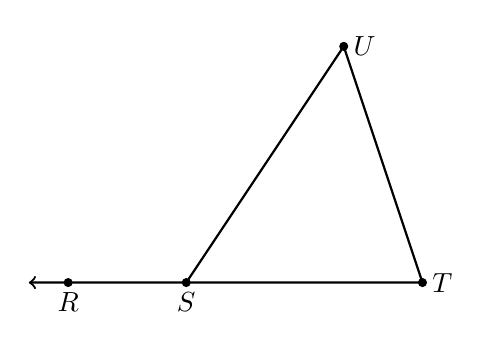
\begin{tikzpicture}
      %\draw [->, thick] (0,0)--(5,5);
      \draw [<-, thick] (-2,0)--(3,0)--(2,3)--(0,0);
      \draw [fill] (-1.5,0) circle [radius=0.05] node[below]{$R$};
      \draw [fill] (0,0) circle [radius=0.05] node[below]{$S$};
      \draw [fill] (2,3) circle [radius=0.05] node[right]{$U$};
      \draw [fill] (3,0) circle [radius=0.05] node[right]{$T$};
    \end{tikzpicture}
    \end{center}

    \item Identify three rays in the given plane.\\[0.25in]
      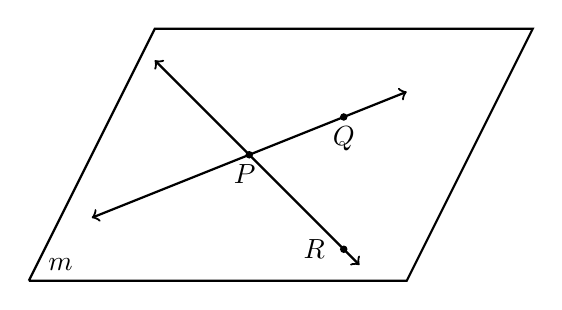
\begin{tikzpicture}[scale=0.8]
        \draw [thick](0,0) node[above right]{$\ m$} --(6,0)--(8,4)--(2,4)--(0,0);
        \draw [<->, thick] (1,1)--(6,3);
        \draw [fill] (3.5,2) circle [radius=0.05] node[below]{$P \ $};
        \draw [fill] (5,2.6) circle [radius=0.05] node[below]{$Q$};
        \draw [<->, thick] (2,3.5)--(5.25,.25);
        \draw [fill] (5,0.5) circle [radius=0.05] node[left]{$R \ $};
      \end{tikzpicture}
      \vspace{0.5cm}

      \item Given $\overleftrightarrow{QS}$ as shown on the number line. \\[10pt] %\vspace{1cm}
      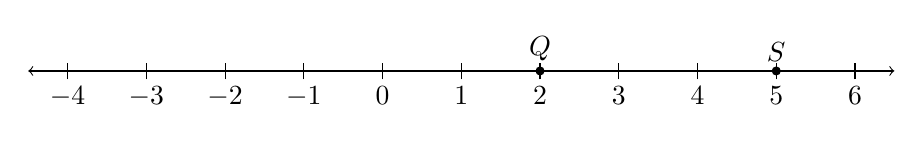
\begin{tikzpicture}
        \draw [<->] (-4.5,0)--(6.5,0);
        \foreach \x in {-4,...,6} %2 leading for diff!=1
          \draw[shift={(\x,0)},color=black] (0pt,-3pt) -- (0pt,3pt) node[below=5pt]  {$\x$};
          \draw [fill] (2,0) circle [radius=0.05] node[above] {$Q$};
          \draw [fill] (5,0) circle [radius=0.05] node[above] {$S$};
      \end{tikzpicture}
      \begin{enumerate}
        \item Mark the point $R$, the midpoint of $\overline{QS}$.
        \item The point $P$ is collinear with $\overleftrightarrow{QS}$ such that $Q$ is the midpoint of $\overleftrightarrow{PS}$. Mark $P$ on the line.
      \end{enumerate}

      \item Points that are all located on the same line are $\rule{4cm}{0.15mm}$.
      \item Find the value of $|3.75 \times (-4)| \div 5$. \vspace{1cm}

      \item Given $\overline{ABC}$, $AC=7 \frac{1}{3}$, and $BC=1 \frac{1}{2}$.
      \begin{enumerate}
        \item Find ${AB}$, expressed as a fraction.\\[0.75cm]
          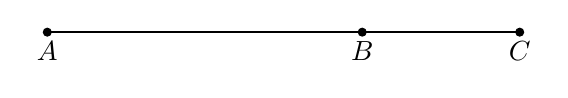
\begin{tikzpicture}
            \draw [-, thick] (1,0)--(7,0);
            \draw [fill] (1,0) circle [radius=0.05] node[below]{$A$};
            \draw [fill] (5,0) circle [radius=0.05] node[below]{$B$};
            \draw [fill] (7,0) circle [radius=0.05] node[below]{$C$};
          \end{tikzpicture} \bigskip
        \item The postulate used in this problem is the \rule{6cm}{0.15mm}.
      \end{enumerate}
      \newpage

      \item Given collinear points $P, Q, R$ with $Q$ bisecting the line segment $\overline{PR}$. $PQ=\frac{1}{3} (x+30)$ and $PR = \frac{7}{3} x$. Find the length of $\overline{PR}$.\\ \bigskip
      First label the drawing.
      \begin{flushright}
      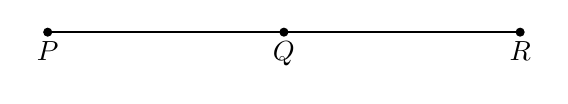
\begin{tikzpicture}
        \draw [-, thick] (0,0)--(6,0);
        \draw [fill] (0,0) circle [radius=0.05] node[below]{$P$};
        \draw [fill] (6,0) circle [radius=0.05] node[below]{$R$};
        \draw [fill] (3,0) circle [radius=0.05] node[below]{$Q$};
      \end{tikzpicture}
      \end{flushright}
      \vspace{1cm}
      \begin{enumerate}
        \item Write a geometric equation: \rule{4cm}{0.15mm} \hspace{1cm} \rule{4cm}{0.15mm}
        \vspace{.7cm}
        \item Substitute algebraic values: \rule{4cm}{0.15mm}
        \item Solve for $x$
        \vspace{4.5cm}
        %\begin{center} $x=$ \rule{1cm}{0.15mm} \end{center}
        \item Answer the question:
        \vspace{2.5cm}
        \item Check your answer
      \end{enumerate}

\end{enumerate}

\end{document}
